% generated by scripts/pkl_to_latex.py
% source PKL : thermal_v1_L6_Ne6_U10_t1_mode-uniform_tpall_t2all_tperpall_nmin2_solver-gcg_full_restarts10_iter300_kmax5_tol1em09_cut10_adaptive1_step5_clusteravg1_T0to1_N20-148a4f8ecb18_knone_diag0.pkl
% scan type  : Tscan
% state      : gs
% quantity   : linear-entropy
% x-max cap  : 0.5
% requires   : \usepackage{pgfplots} \pgfplotsset{compat=1.18}
% colours match the matplotlib PDF (tab10 cycle)
\definecolor{gmeC0}{HTML}{1F77B4}
\definecolor{gmeC1}{HTML}{FF7F0E}
\definecolor{gmeC2}{HTML}{2CA02C}
\definecolor{gmeC3}{HTML}{D62728}
\definecolor{gmeC4}{HTML}{9467BD}
\definecolor{gmeC5}{HTML}{8C564B}
\definecolor{gmeC6}{HTML}{E377C2}
\definecolor{gmeC7}{HTML}{17BECF}

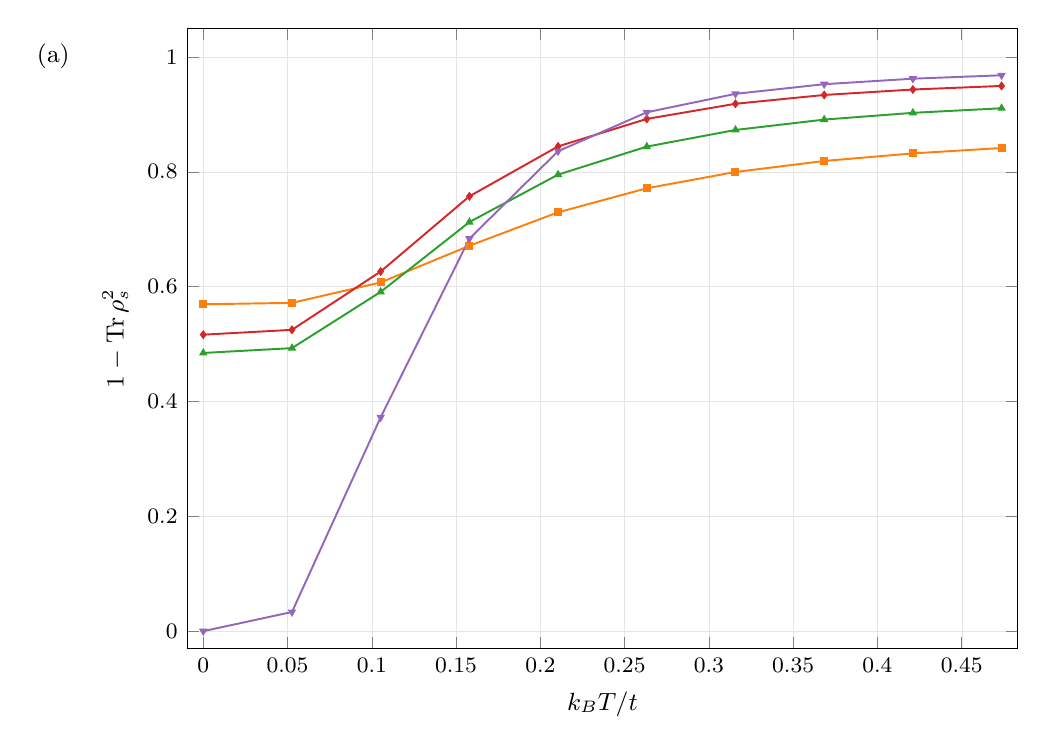
\begin{tikzpicture}
  \begin{axis}[
    width=\columnwidth,
    height=0.78\columnwidth,
    xlabel={$k_B T/t$},
    ylabel={$1-\mathrm{Tr}\,\rho_s^2$},
    grid=both,
    grid style={line width=.1pt, draw=gray!20},
    tick label style={font=\footnotesize\rmfamily, /pgf/number format/fixed},
    label style={font=\small\rmfamily},
    scaled ticks=false,
    legend style={font=\scriptsize\rmfamily, draw=gray!40, at={(0.5,1.03)}, anchor=south, /tikz/every even column/.append style={column sep=6pt}},
    legend cell align={left},
    legend columns=2,
    ymin=-0.03,
    ymax=1.05,
    xmin=-0.00947368,
    xmax=0.483158,
    after end axis/.append code={\node[anchor=east, font=\small\rmfamily] at (axis description cs:-0.13,0.954) {(a)};},
  ]
    \addplot[color=gmeC1, mark=square*, mark size=1.1pt, line width=0.7pt] coordinates {
        (0,0.569263) (0.052632,0.571733) (0.105263,0.607328) (0.157895,0.67116)
        (0.210526,0.729423) (0.263158,0.771312) (0.315789,0.799652) (0.368421,0.81882)
        (0.421053,0.832035) (0.473684,0.841375)
    };
    \addplot[color=gmeC2, mark=triangle*, mark size=1.1pt, line width=0.7pt] coordinates {
        (0,0.484489) (0.052632,0.492905) (0.105263,0.59086) (0.157895,0.712419)
        (0.210526,0.795051) (0.263158,0.843817) (0.315789,0.872826) (0.368421,0.890867)
        (0.421053,0.902632) (0.473684,0.910636)
    };
    \addplot[color=gmeC3, mark=diamond*, mark size=1.1pt, line width=0.7pt] coordinates {
        (0,0.516315) (0.052632,0.524765) (0.105263,0.626356) (0.157895,0.757242)
        (0.210526,0.844189) (0.263158,0.892064) (0.315789,0.918423) (0.368421,0.933763)
        (0.421053,0.943262) (0.473684,0.949477)
    };
    \addplot[color=gmeC4, mark=triangle*, mark size=1.1pt, mark options={rotate=180}, line width=0.7pt] coordinates {
        (0,0) (0.052632,0.03339) (0.105263,0.372497) (0.157895,0.683464)
        (0.210526,0.835799) (0.263158,0.903592) (0.315789,0.935726) (0.368421,0.952512)
        (0.421053,0.962116) (0.473684,0.968041)
    };
  \end{axis}
\end{tikzpicture}
